%===============================================================================================
%		Referenzbeispiele
%===============================================================================================

\chapter{Referenzbeispiele}
\label{sec:ReferenceExamples}

Um die Erf�llung der \LibName{}-Anforderungen sicherzustellen, wird eine Menge von (gr��tenteils) real-life Beispielen f�r alle unterst�tzten Formate definiert. Diese Beispiele werden benutzt, um Designentscheidungen zu illustieren, aber auch um sie zu verifizieren. In diesem Kapitel werden diese Beispiele in K�rze definiert. Die detaillierte Struktur jedes verwendeten Datenformats wird in \cite{MetaComp} behandelt.

Wichtig: Die Gr��en der Datenbl�cke in den folgenden Abbildungen haben keine Bedeutung.

%-----------------------------------------------------------------------------------------------
%		Beispiel 1: MP3 File mit ID3v2.3, ID3v1.1 und Lyrics3
%-----------------------------------------------------------------------------------------------

\section{Beispiel 1: MP3 File mit ID3v2.3, ID3v1.1 und Lyrics3}
\label{sec:Example1MP3FileWithID3v23AndID3v11}

Die folgende Abbildung zeigt das erste Beispiel, eine MP3-Datei mit drei \TERMtag{}s, ID3v2.3, Lyrics3v2 und ID3v1.1. Alle befinden sich am Ende der Datei:

\begin{figure}[H]
	\centering
	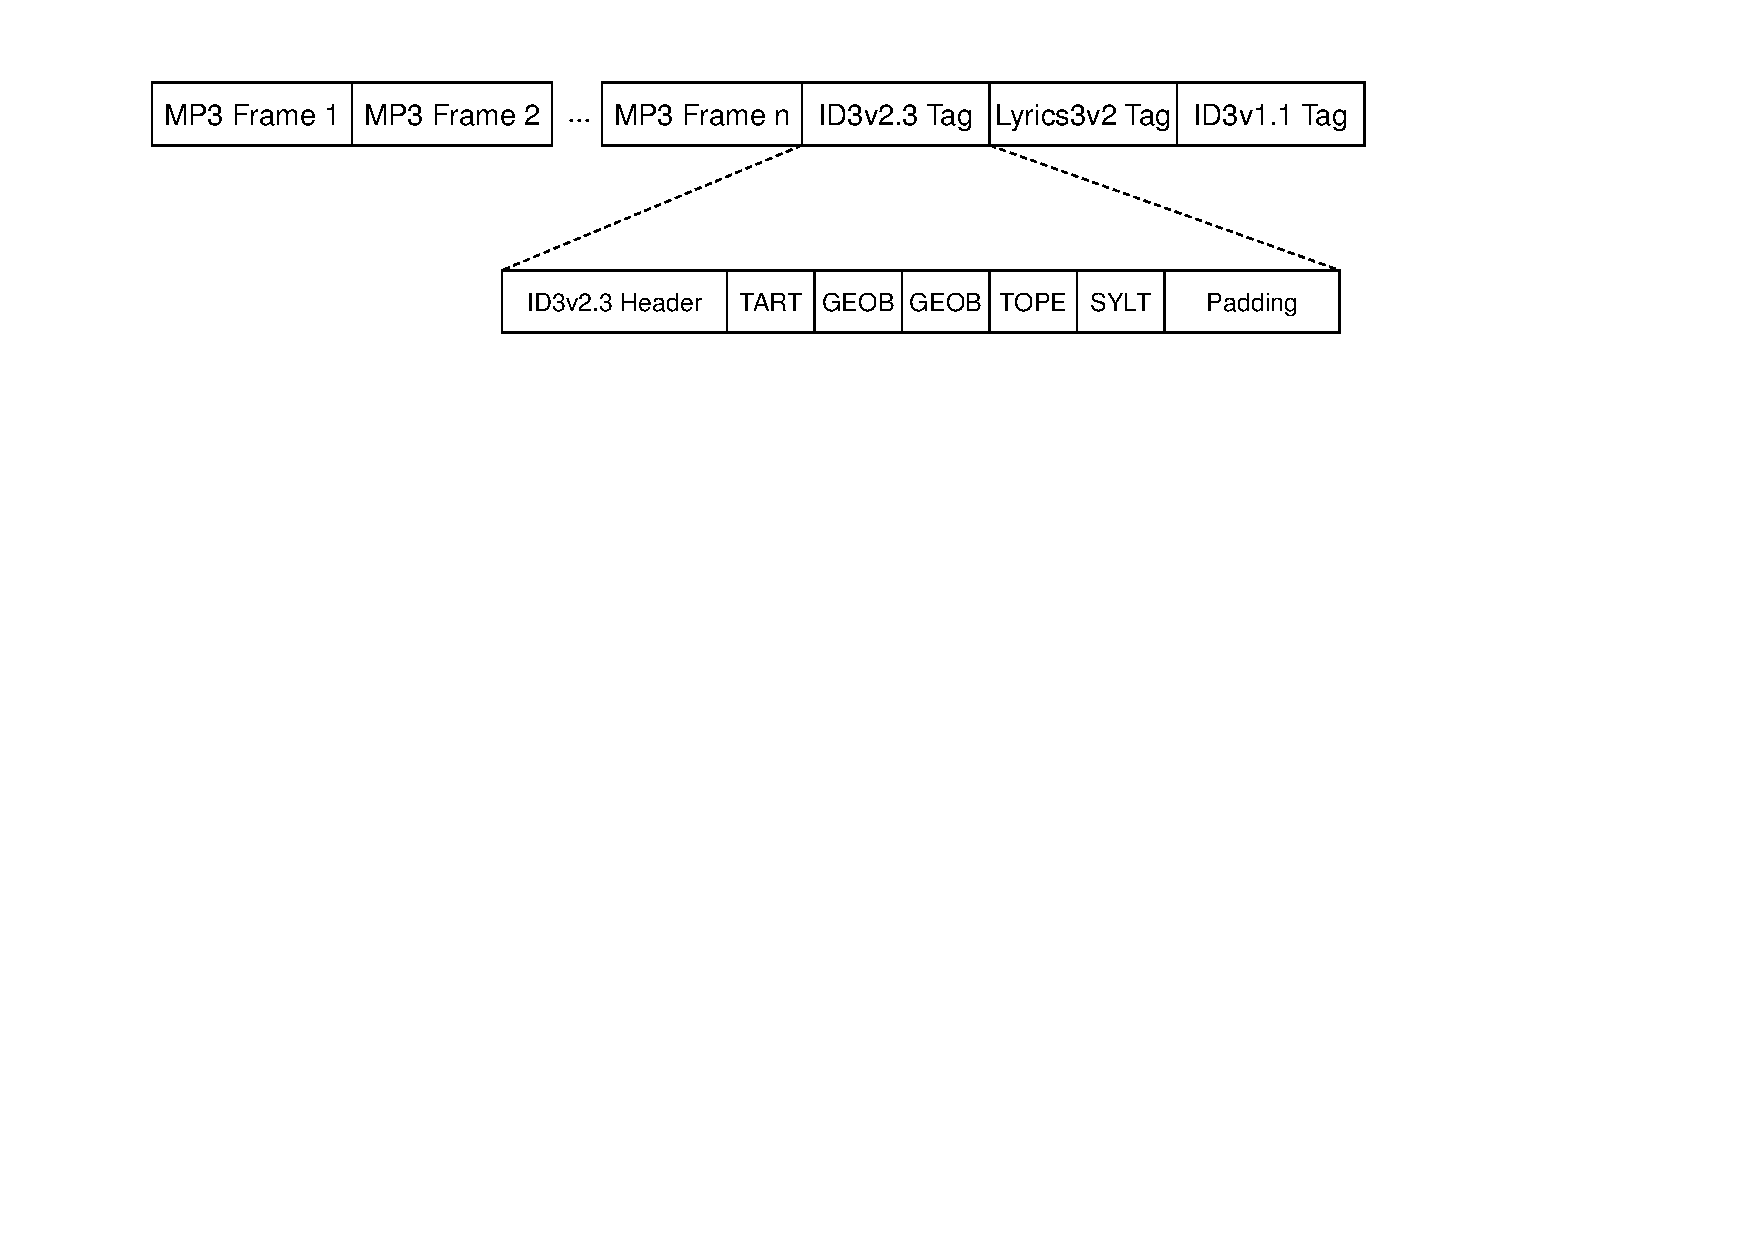
\includegraphics[width=1.00\textwidth]{Figures/Part_I/I_5_Example1.pdf}
	\caption{Beispiel 1: MP3 File mit ID3v2.3, ID3v1.1 und Lyrics3}
	\label{fig:Example1MP3filewithtwotags}
\end{figure}

Das ID3v2.3-\TERMtag{} hat mehrere Frames, einen \texttt{GEOB}-Frame inbegriffen. Weiterhin hat es ein wenig Padding am Ende. Jeder der MP3-Frames korrespondiert zu einem MPEG-1 ``elementary stream audio format''.

%-----------------------------------------------------------------------------------------------
%		Beispiel 2: MP3 File mit zwei ID3v2.4 Tags
%-----------------------------------------------------------------------------------------------

\section{Beispiel 2: MP3 File mit zwei ID3v2.4 Tags}
\label{sec:Example2MP3FileWithID3v23AndID3v11}

Die folgende Abbildung zeigt das zweite Beispiel, eine MP3-Datei mit zwei ID3v2.4 \TERMtag{}s, eines am Anfang, das andere am Ende der Datei:

\begin{figure}[H]
	\centering
	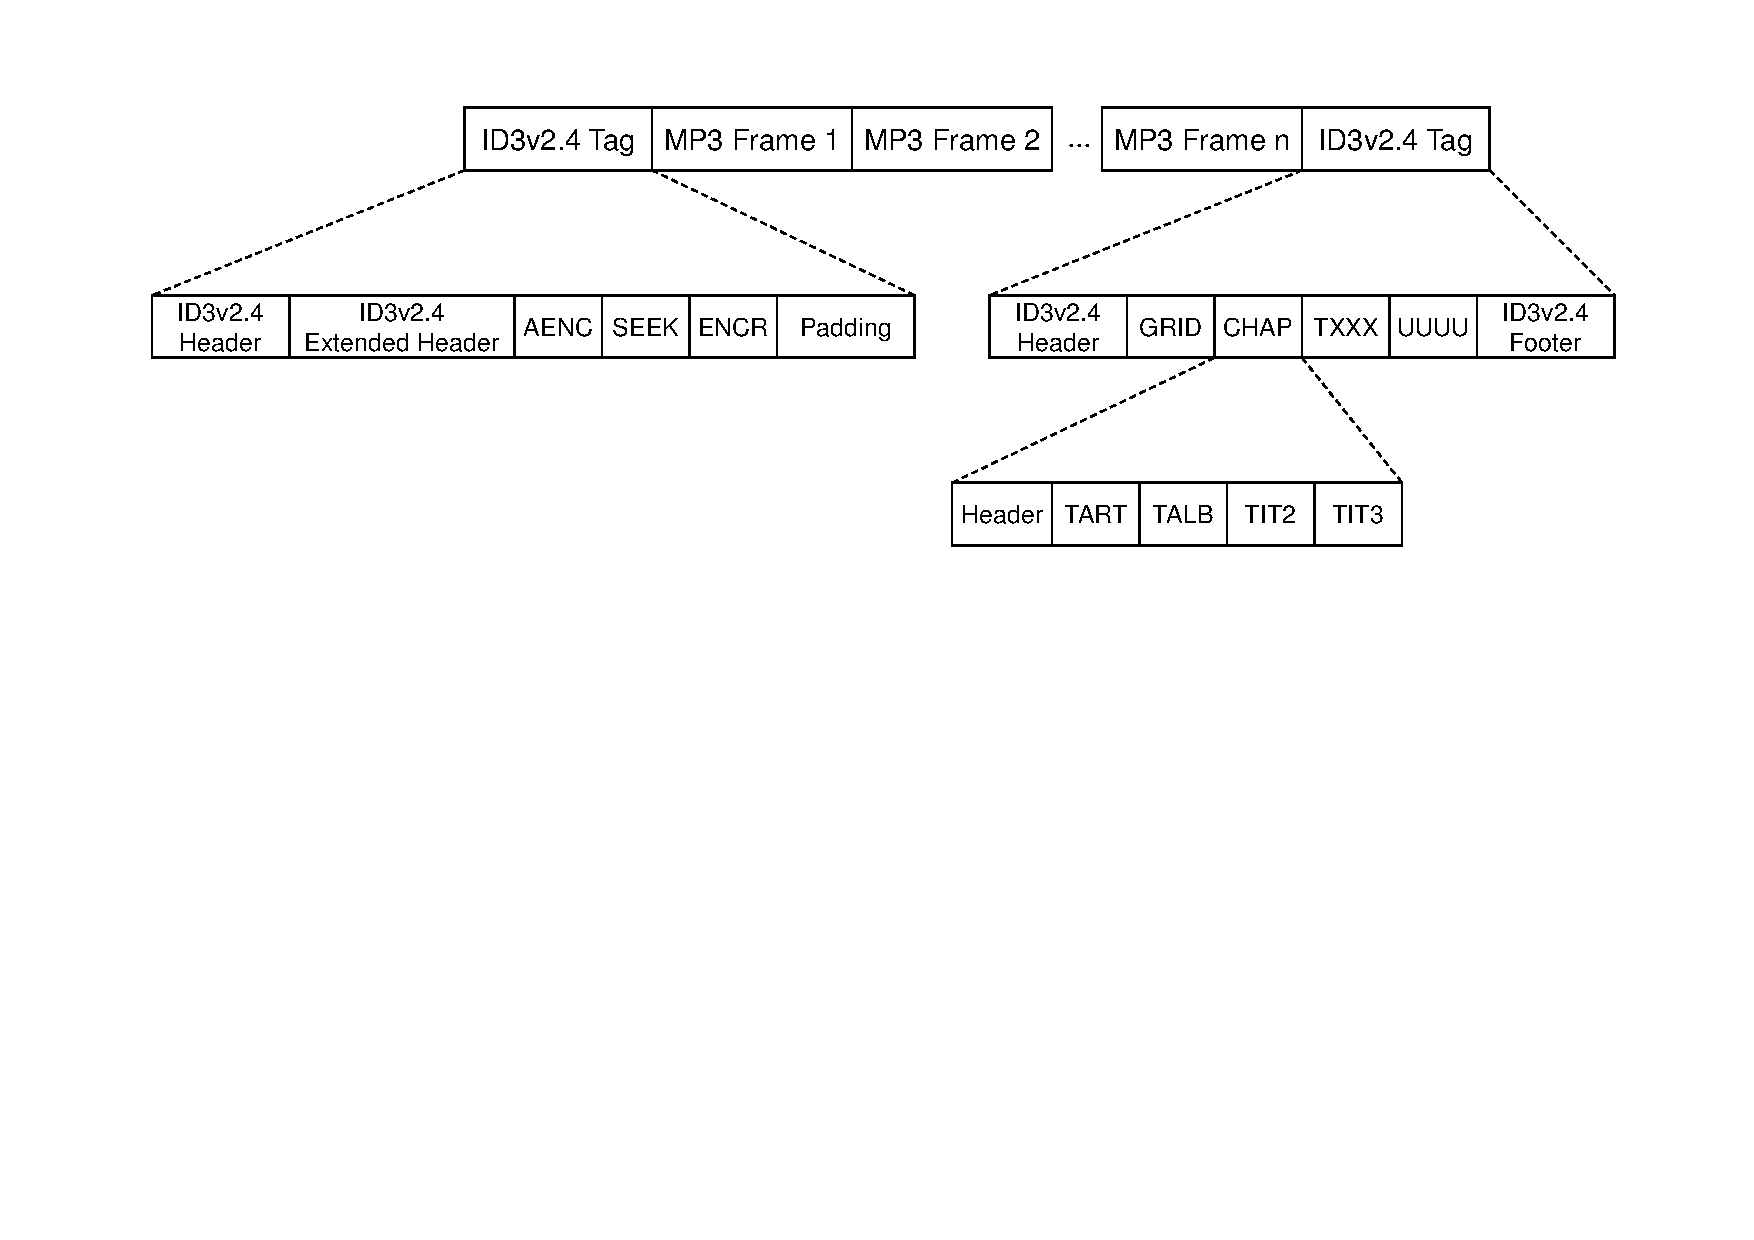
\includegraphics[width=1.00\textwidth]{Figures/Part_I/I_5_Example2.pdf}
	\caption{Beispiel 2: MP3 File mit zwei ID3v2.4 Tags}
	\label{fig:Example1MP3filewithtwoID3tags}
\end{figure}

Die zwei ID3v2.4 \TERMtag{}s sind virtuell �ber einen \texttt{SEEK}-Frame verbunden. Beide haben verschiedene Spezialit�ten, die in \cite{MetaComp} beschrieben sind.

%-----------------------------------------------------------------------------------------------
%		Beispiel 3: Ogg Bitstream mit Theora und VorbisComment
%-----------------------------------------------------------------------------------------------

\section{Beispiel 3: Ogg Bitstream mit Theora und VorbisComment}
\label{sec:Example4MP3FileWithID3v23AndID3v11}

Die folgende Abbildung zeigt das dritte Beispiel, einen Ogg bitstream der Theora als Nutzdaten enth�lt, mit einem Vorbis comment:

\begin{figure}[H]
	\centering
	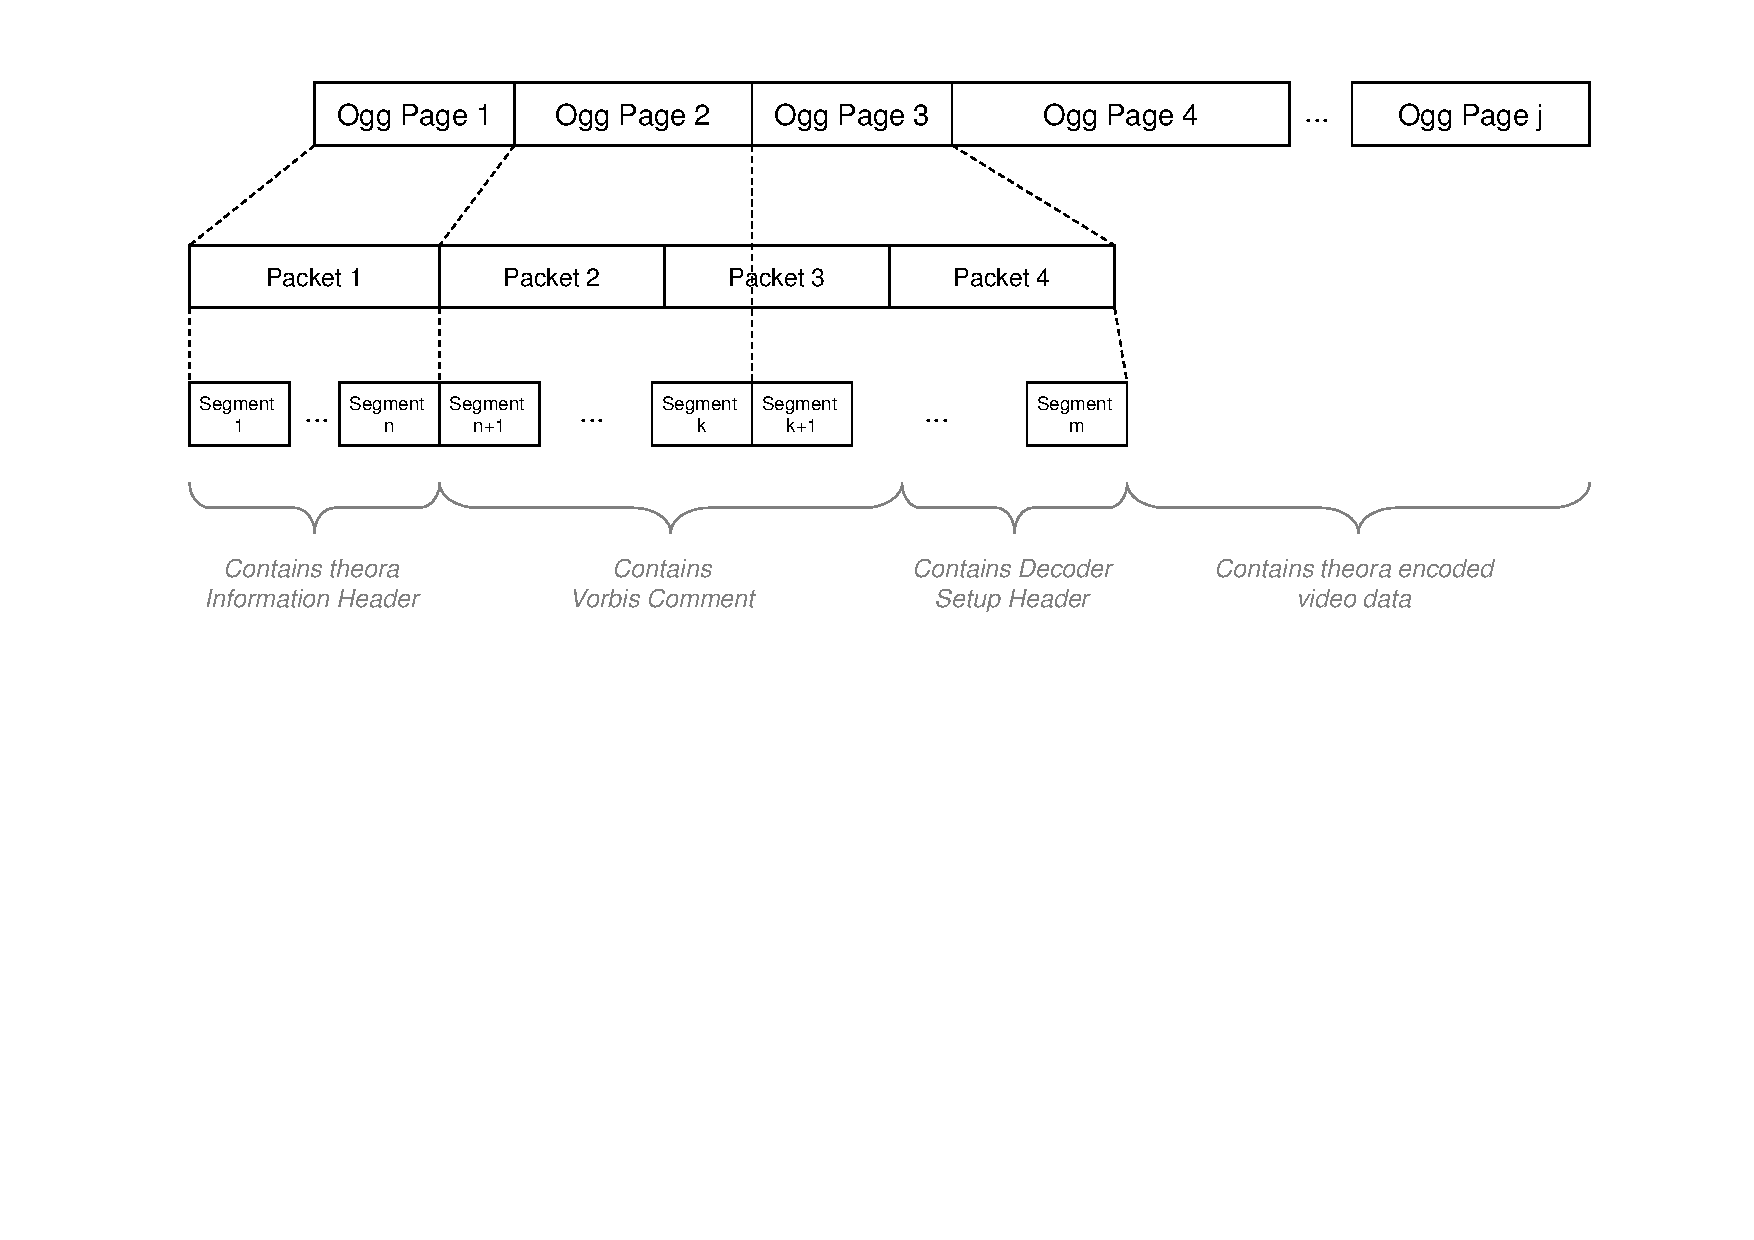
\includegraphics[width=1.00\textwidth]{Figures/Part_I/I_5_Example4.pdf}
	\caption{Beispiel 4: Ogg Bitstream mit Theora und VorbisComment}
	\label{fig:Example4MP3filewithtwoID3tags}
\end{figure}

Das Beispiel scheint auf den ersten Blick komplex zu sein. In einem Ogg bitstream sind physikalische und logische  Struktur nicht notwendigerweise das gleiche. Die physikalische Strukture wird durch pages, packets und segments gebildet, w�hrend die logische  Struktur die struktur der gewrappten Daten ist. Wir haben hier theora als Video-Daten-Beispiel verwendet, aber dies ist prinzipiell beliebig, weil der Codec f�r \LibName{} keine Rolle spielt. Was aber eine Rolle spielt ist die Position des Vorbis Comment, eines der unterst�tzten Datenformate. Dies h�ngt jedoch ungl�cklicherweise vom gespeicherten Codec ab. In diesem Beispiel startet der vorbis comment in der zweiten Page und �berspannt zwei packets. Das zweite dieser Packets �berspannt zwei Ogg pages.

%%% Hinweis: Die folgenden Sektionen sind auskommentiert, da diese Formate noch nicht in v0.5 der Library
%%%   relevant sind.
%
%%-----------------------------------------------------------------------------------------------
%%		Beispiel 4: TIFF RGB Bild-Datei mit EXIF IFD
%%-----------------------------------------------------------------------------------------------
%
%\section{Beispiel 4: TIFF RGB Bild-Datei mit EXIF IFD}
%\label{sec:Example5MP3FileWithID3v23AndID3v11}
%
%Eine Beispiel TIFF RGB Bild-Datei mit einem Exif IFD wird in der folgenden Abbildung dargestellt:\footnote{Das Beispiel basiert auf der Abbildung in \cite{ExifSpec}, Seite 9.}
%
%\begin{figure}[H]
	%\centering
	%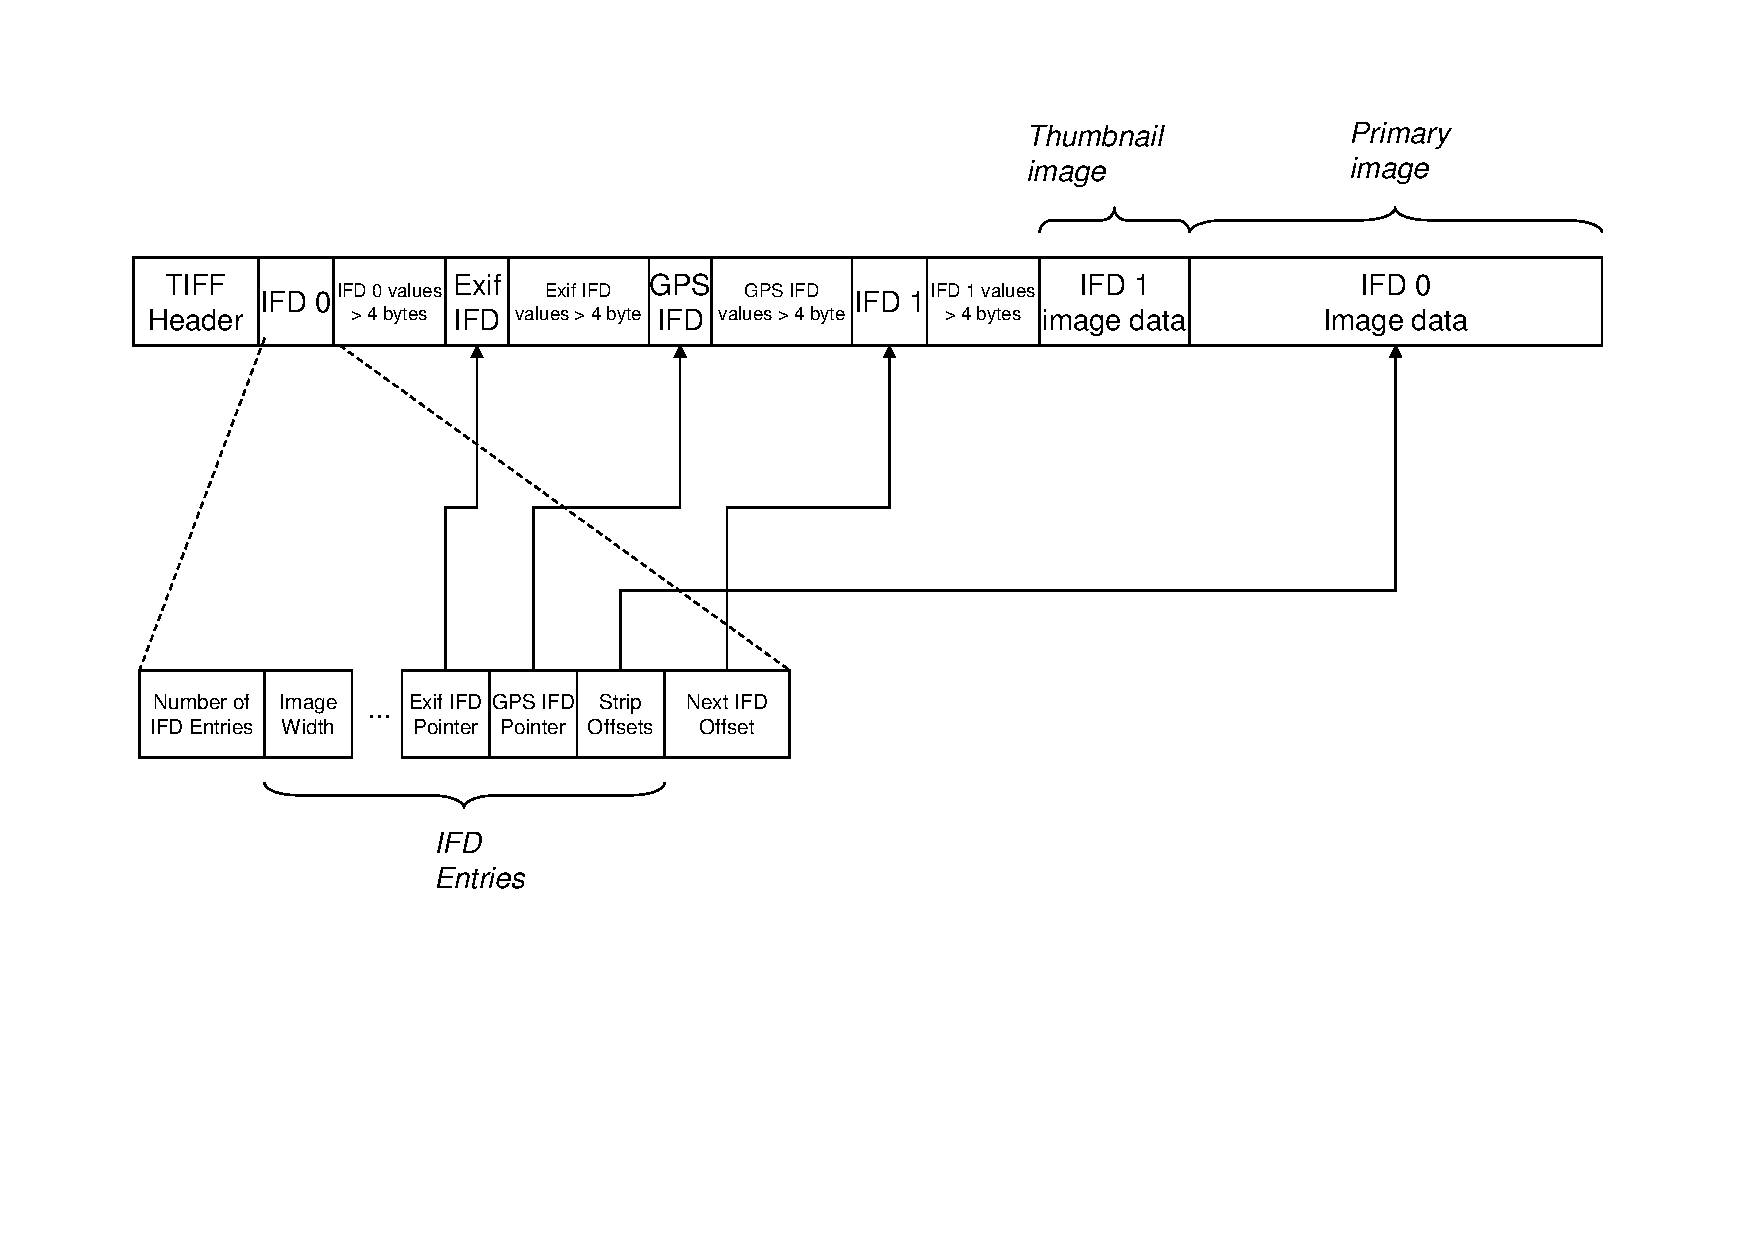
\includegraphics[width=1.00\textwidth]{Figures/Part_I/I_5_Example5.pdf}
	%\caption{Beispiel 4: TIFF RGB Bild-Datei mit EXIF IFD}
	%\label{fig:Example5MP3filewithtwoID3tags}
%\end{figure}
%
%Das Beispiel enth�lt zwei Bilddaten-Anteile, die hier direkt hintereinander gespeichert sind. Der erste Teil ist nur ein Thumbnail-Bild, w�hrend das zweite die echtne Bilddaten speichert. Die Abbildung zeigt die verpointerte  Struktur der Datei, weil IFD-Felder h�ufig auf Byte-Offsets verweisen, an denen die tats�chlichen Bilddaten gespeichert sind.
%
%%-----------------------------------------------------------------------------------------------
%%		Beispiel 5: RIFF-WAVE-Datei
%%-----------------------------------------------------------------------------------------------
%
%\section{Beispiel 5: RIFF-WAVE-Datei}
%\label{sec:Example6MP3FileWithID3v23AndID3v11}
%
%Eine Beispiel-RIFF-WAVE-Datei mit einem Exif IFD wird in der folgenden Abbildung dargestellt:
%
%\begin{figure}[H]
	%\centering
	%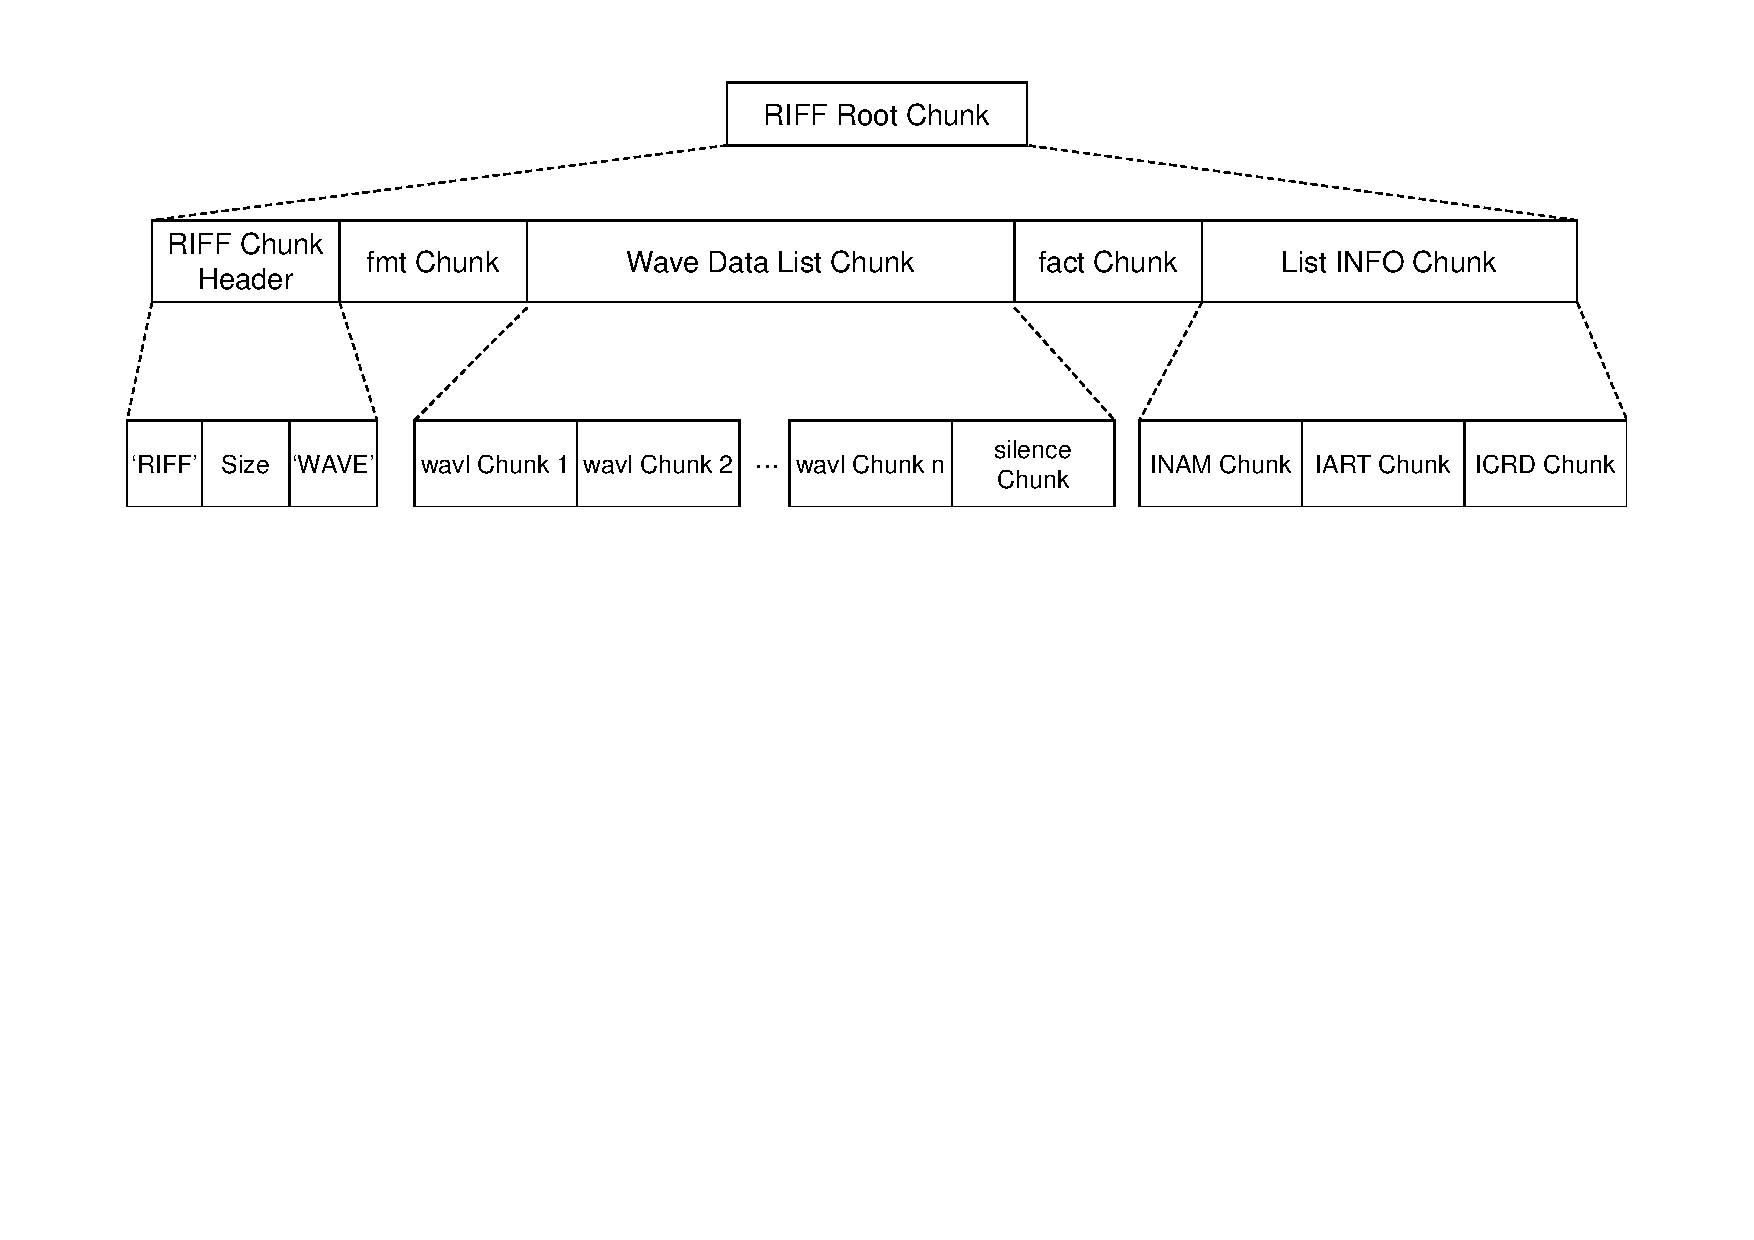
\includegraphics[width=1.00\textwidth]{Figures/Part_I/I_5_Example6.pdf}
	%\caption{Beispiel 5: RIFF-WAVE-Datei}
	%\label{fig:Example6MP3filewithtwoID3tags}
%\end{figure}
%
%Der top-level root-Chunk enth�lt einen fact-Chunk, einen format-Chunk, eine Liste von Wave-data-Chunks und schlie�lich einen \texttt{LIST}-info-Chunk in seinen Nutzdaten. Der \texttt{LIST}-info-Chunk kann als \TERMtag{} betrachtet werden. Er enth�lt die \texttt{INAM}, \texttt{IART} und \texttt{ICRD} Sub-Chunks.
%
%%-----------------------------------------------------------------------------------------------
%%		Beispiel 6: QuickTime-Datei
%%-----------------------------------------------------------------------------------------------
%
%\section{Beispiel 6: QuickTime-Datei}
%\label{sec:Example7MP3FileWithID3v23AndID3v11}
%
%Eine Beispiel-QuickTime-Datei mit einem Exif IFD wird in der folgenden Abbildung dargestellt:
%
%\begin{figure}[H]
	%\centering
	%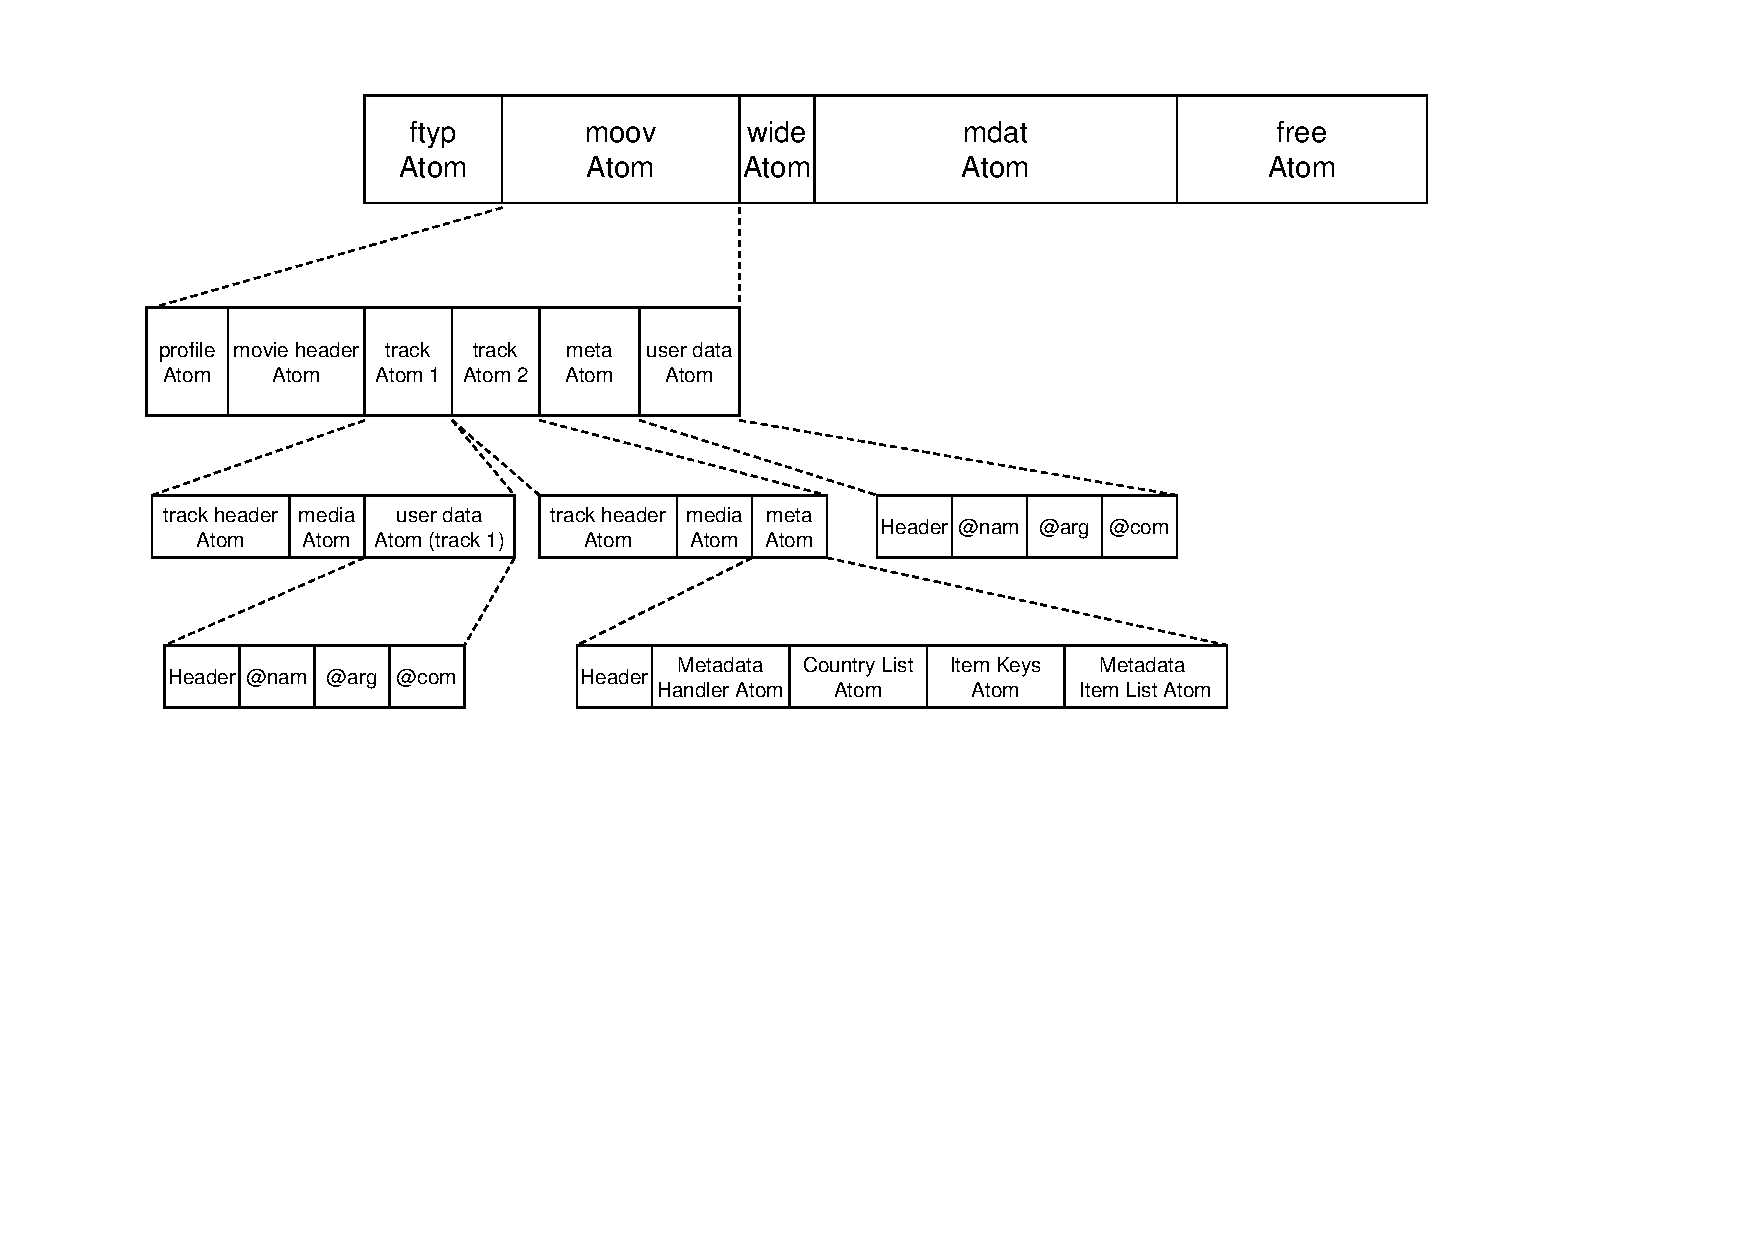
\includegraphics[width=1.00\textwidth]{Figures/Part_I/I_5_Example7.pdf}
	%\caption{Beispiel 6: QuickTime-Datei}
	%\label{fig:Example7MP3filewithtwoID3tags}
%\end{figure}
%
%Eine QuickTime-Datei kann leicht sehr komplex werden. Das Beispiel enth�lt die Atoms \texttt{ftyp}, \texttt{moov}, \texttt{mdat} und \texttt{free} als top-level Atoms. Das \texttt{mdat} Atom enth�lt Medien-Daten und wird in diesem Beispiel nicht weiter ausdetailliert. Es wird gefolgt von einem nachgelagerten wide-Atom, um einfache Erweiterbarkeit auf einen Header zu erm�glichen, der mehr als $2^{32}$ Bytes als Gr��e des media Atoms angeben kann.
%
%Das Beispiel definiert zwei tracks im movie Atom. Eines enth�lt weiterhin ein user data Atom, das Key-Value Metadaten enth�lt. Der andere track enth�lt das QuickTime \texttt{meta} Atom, das ebenso Metadaten definiert, aber auf unterschiedliche Art und Weise.
%
%Das Beispiel zeigt, dass das \texttt{moov} Atom selbst zus�tzlich ein \texttt{meta} und ein user data Atom enthalten kann, welche die gesamte Datei beschreiben.
%
%%-----------------------------------------------------------------------------------------------
%%		Beispiel 8: Matroska-Datei
%%-----------------------------------------------------------------------------------------------
%
%\section{Beispiel 7: Matroska-Datei}
%\label{sec:Example8MP3FileWithID3v23AndID3v11}
%
%Eine Beispiel-Matroska-Datei mit einem Exif IFD wird in der folgenden Abbildung dargestellt:
%
%\begin{figure}[H]
	%\centering
	%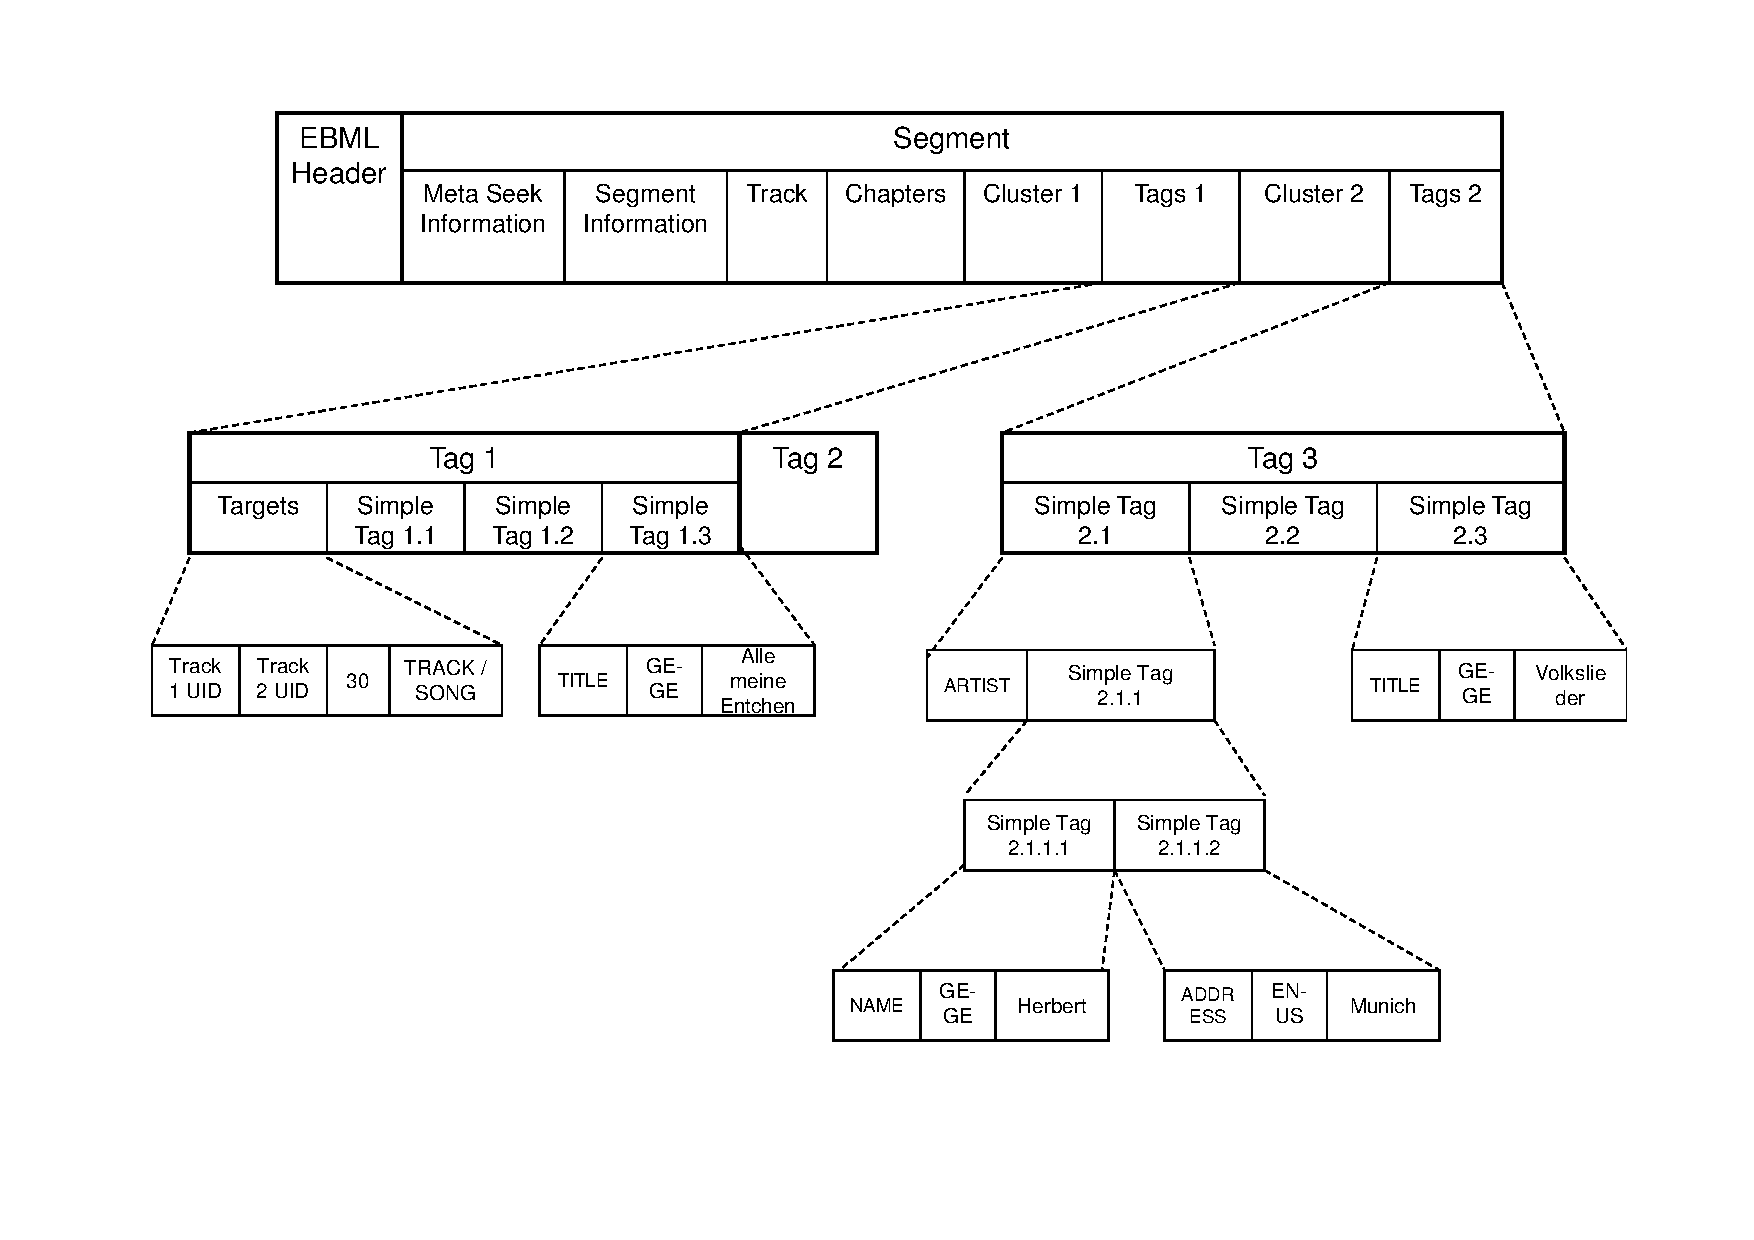
\includegraphics[width=1.00\textwidth]{Figures/Part_I/I_5_Example8.pdf}
	%\caption{Beispiel 7: Matroska-Datei}
	%\label{fig:Example8MP3filewithtwoID3tags}
%\end{figure}
%
%Das Beispiel hat zwei Cluster Elemente die die tats�chlichen Medien-Daten enthalten. Diese werden im Beispiel nicht weiter ausdetailliert. Die Metadaten dieses Beispiels sind komplex: Es gibt zwei top-level Tags Elemente, das erste enth�lt zwei weitere Tag Elemente, das zweite nur ein weiteres Tag Element. Jedes der Tag-Elemente hat als Kind ein SimpleTag Element. Das erste Tag enth�lt das Targets Sub-element, das auf zwei Tracks der Datei verweist. Tag 3 enth�lt nur SimpleTags. Jedoch enth�lt das erste SimpleTag eingebettete SimpleTags.

%###############################################################################################
%###############################################################################################
%
%		File end
%
%###############################################################################################
%###############################################################################################